% Poster draft, CSC2529 poster session (Dec 2).  Build:  cd poster && tectonic poster.tex
% Grey dashed boxes are placeholders. Each names the workstream in docs/PLAN.md that fills it.
% Real numbers so far: Stage 2 checker study (docs/STAGE2.md, PR #9) and cadrille's baseline.
\documentclass[25pt, a0paper, landscape, margin=0mm, innermargin=12mm,
  blockverticalspace=9mm, colspace=10mm, subcolspace=6mm]{tikzposter}

\usepackage[T1]{fontenc}
\usepackage{helvet}
\renewcommand{\familydefault}{\sfdefault}
\usepackage{amsmath,amssymb}
\usepackage{graphicx}
\usepackage{booktabs}
\usepackage{tabularx}
\usepackage{enumitem}
\setlist{leftmargin=1.2em, itemsep=3pt, topsep=3pt}
\usetikzlibrary{positioning, arrows.meta, calc}
\graphicspath{{figures/}}

% ------------------------------------------------------------------ look
\definecolorstyle{Draft}{
  \definecolor{colorOne}{HTML}{1E3765}    % dark blue: titles
  \definecolor{colorTwo}{HTML}{2A78D6}    % blue: same as "weights on" in the Stage 2 figures
  \definecolor{colorThree}{HTML}{EB6834}  % orange: accents, callouts
}{
  \colorlet{backgroundcolor}{white}
  \colorlet{framecolor}{colorOne}
  \colorlet{titlefgcolor}{white}
  \colorlet{titlebgcolor}{colorOne}
  \colorlet{blocktitlebgcolor}{colorOne}
  \colorlet{blocktitlefgcolor}{white}
  \colorlet{blockbodybgcolor}{white}
  \colorlet{blockbodyfgcolor}{black}
  \colorlet{innerblocktitlebgcolor}{colorTwo}
  \colorlet{innerblocktitlefgcolor}{white}
  \colorlet{innerblockbodybgcolor}{colorTwo!7}
  \colorlet{innerblockbodyfgcolor}{black}
  \colorlet{notefgcolor}{black}
  \colorlet{notebgcolor}{colorThree!10}
  \colorlet{noteframecolor}{colorThree}
}
\usetheme{Default}
\usecolorstyle{Draft}
\usetitlestyle{Filled}
\useblockstyle{Default}

% A dashed grey box standing in for a result that does not exist yet.
%   \placeholder{<height>}{<what it will show>}{<details: data, source workstream>}
\newcommand{\placeholder}[3]{%
  \begin{tikzpicture}
    \node[draw=black!35, dashed, line width=2pt, fill=black!4, rounded corners=8pt,
          minimum width={\linewidth-6pt}, minimum height=#1, inner sep=12pt,
          text width={\linewidth-70pt}, align=center, text=black!65]
      {\textbf{Placeholder: #2}\\[6pt]{\small #3}};
  \end{tikzpicture}}

\newcommand{\pending}[1]{\textcolor{colorThree}{\textbf{[#1]}}}

% ------------------------------------------------------------------ title
% (a line break directly in \title breaks tikzposter's title node; keep the \parbox)
\title{\parbox{0.8\paperwidth}{\centering Agentic VLM Visual Review and
       Forward-Rendering Geometric Checks\\ for Iterative Image-to-CAD Reconstruction}}
\author{Miran Qarachatani \quad Teodor Cirstoiu \quad Metom Bega}
\institute{University of Toronto \,\textbullet\, CSC2529 Computational Imaging, Fall 2026
  \qquad \textcolor{colorThree!60!white}{\textbf{DRAFT: grey dashed boxes are placeholders}}}

\tikzposterlatexaffectionproofoff
\begin{document}
\maketitle

\begin{columns}
% ================================================================== column 1: why + how
\column{0.25}

\block{The question}{
  Single-pass image-to-CAD models miss features. VLM agents can refine 3D models from
  renders \cite{gator,cadcodeverify} but judge their own edits by eye. GATOR \cite{gator}
  calls \emph{automatic geometric verification} and \emph{robustness to imperfect
  observations} open problems.

  \vspace{6pt}
  \textbf{We ask:}
  \begin{enumerate}
    \item Do forward-rendering checks guide and judge CAD edits better than VLM visual
          review?
    \item Do they still work when masks and depth are wrong?
  \end{enumerate}
}

\block{Image-to-CAD as an inverse problem}{
  The unknown is a CadQuery program $\theta$. The forward model builds the solid and
  renders silhouettes $\hat S_v(\theta)$ and depth $\hat D_v(\theta)$ from 8 calibrated
  cameras. The measurements are the target's $S_v$ and $D_v$.

  \vspace{6pt}
  \textbf{Score} (no 3D ground truth):
  \[
    \mathrm{geo}(\theta)=\sum_v \bar w_v\,\mathrm{IoU}\big(\hat S_v,S_v\big)
      -\sum_v \bar w_v\,\mathrm{MAE}\big(\hat D_v,D_v\big)
  \]
  \textbf{Gate:} keep an edit only if $\mathrm{geo}$ rises by more than $10^{-3}$ and no
  trusted view ($w_v \ge 0.5$) loses more than $0.05$ IoU.

  \vspace{6pt}
  \textbf{View weights} (space carving): every view's depth is back-projected and checked
  by the others; $r(v,u)$ is the mutual rejection rate.
  \[
    c_v = 1-\operatorname{median}_u r(v,u),\qquad
    w_v = \mathrm{clip}\!\left(\tfrac{c_v-0.6}{0.38},0,1\right)
  \]
  A view that disagrees with the rest counts less and cannot veto an edit.
}

\block{Setup}{
  \begin{itemize}
    \item \textbf{60 Fusion360 test parts}, stratified by cadrille IoU $\times$ mesh
          complexity; 18 separate tuning parts for design choices.
    \item \textbf{Start:} cadrille's RL program \cite{cadrille}; on 345 Fusion360 test
          parts: median 3D IoU 93.7\%, mean 84.5\%.
    \item \textbf{Agent:} Gemini 3.8 Flash; Gemma 4 12B (open weights).
    \item \textbf{Cameras:} 6 axis + 2 isometric views, $512\times512$ px.
    \item \textbf{Metrics} vs.\ hidden ground truth: 3D IoU, Chamfer, kept edits that
          helped or harmed, cost per part.
  \end{itemize}
}

% ================================================================== column 2: the loop
\column{0.25}

\block{The refinement loop}{
  \begin{center}
  \begin{tikzpicture}[
      node distance=20mm and 30mm,
      box/.style={draw=colorOne, line width=2pt, rounded corners=8pt, fill=white,
                  align=center, text width=9.2cm, minimum height=3.0cm, inner sep=7pt},
      start/.style={box, fill=colorTwo!10, text width=20cm, minimum height=2.2cm},
      gate/.style={box, draw=colorThree, fill=colorThree!10},
      arr/.style={-{Stealth[length=6mm, width=5mm]}, line width=2.5pt, draw=colorOne},
      lab/.style={font=\small, text=colorOne, fill=white, inner sep=3pt}]
    \node[box] (prog) {\textbf{Program} $\theta_t$\\{\small CadQuery code}};
    \node[box, right=of prog] (cmp) {\textbf{Render and compare}\\{\small 8 views vs.\
      target silhouettes + depth}};
    \node[box, below=of cmp] (agent) {\textbf{Agent edits}\\{\small sees renders,
      residual images, per-view table}};
    \node[gate, below=of prog] (gate) {\textbf{Gate}\\{\small geometric check (geo)
      or VLM judge}};
    \node[start, above=18mm of $(prog.north)!0.5!(cmp.north)$] (start)
      {Input: 8 calibrated views $\;\to\;$ cadrille writes the first program};
    \draw[arr] (start.south -| prog.north) -- (prog.north);
    \draw[arr] (prog) -- node[lab, above=4pt] {build} (cmp);
    \draw[arr] (cmp) -- node[lab, right=4pt, align=left] {residuals} (agent);
    \draw[arr] (agent) -- node[lab, below=4pt] {edit $\theta'$} (gate);
    \draw[arr] (gate) -- node[lab, left=4pt, align=right] {keep $\theta'$\\or revert} (prog);
  \end{tikzpicture}
  \end{center}

  \vspace{4pt}
  \small
  \begin{tabularx}{\linewidth}{@{}l X X@{}}
    \toprule
    \textbf{Arm} & \textbf{Agent also sees} & \textbf{Edit kept if} \\
    \midrule
    premise & target + current renders & VLM judge prefers it \\
    vlm & + failed visual questions \cite{cadcodeverify} & VLM judge prefers it \\
    \textbf{geo (ours)} & + residual images, per-view table & geometric gate passes \\
    hybrid & everything above & gate \emph{and} judge \\
    oracle & as geo & hidden 3D IoU rises \\
    \bottomrule
  \end{tabularx}
}

\block{What the checker sees}{
  \begin{center}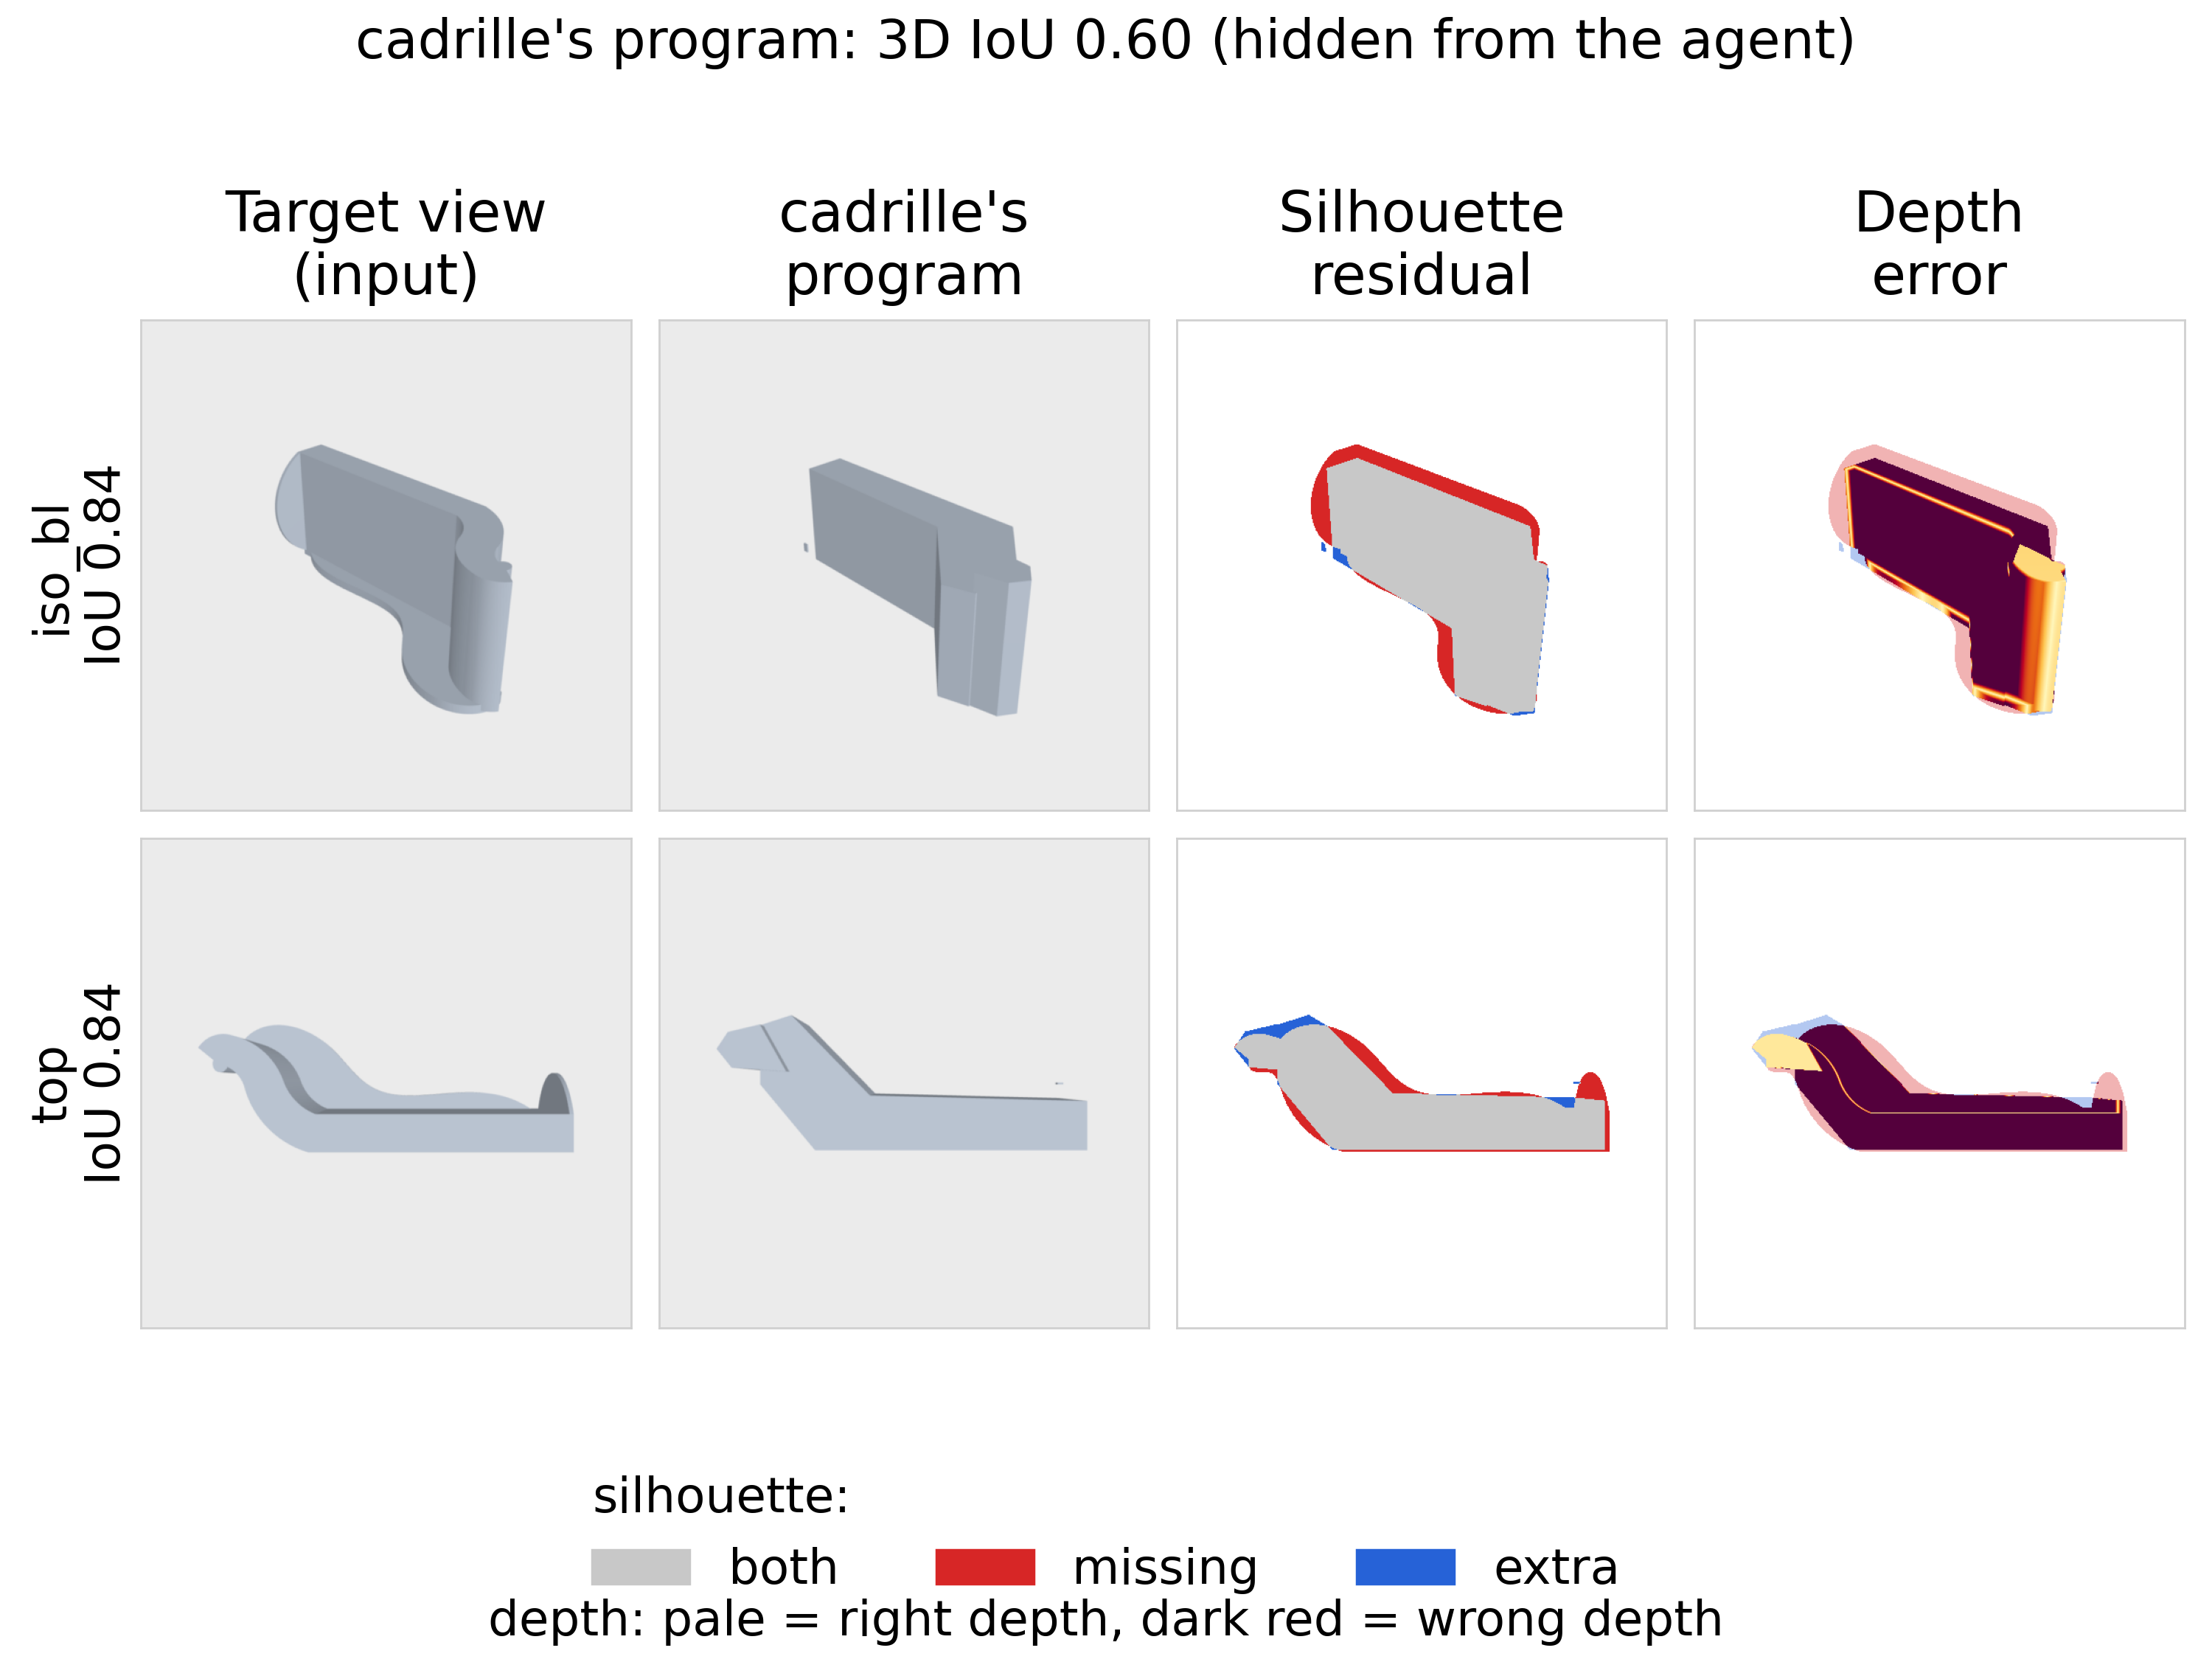
\includegraphics[width=0.9\linewidth]{checker_example.png}\end{center}\vspace{-10pt}

  {\small Two of the 8 views of one Stage 1 part. In the geo arm the agent gets these
  residuals and a per-view table every round.}
}

\block{Real photos}{
  \placeholder{5cm}{SAM 3 masks and VGGT depth \cite{sam3,vggt}}{Where the errors of
    masks and depth estimated from RealCAD photos sit on the Stage 2 curves. Source: W6.}
}

% ================================================================== column 3: Stage 1
\column{0.25}

\block{Stage 1: clean views}{
  \placeholder{10.5cm}{3D IoU gain over cadrille, per arm}{Paired gain (final $-$ start)
    with 95\% bootstrap CI over the 56 parts with watertight ground truth, by cadrille IoU
    bin. Source: W1, due Nov 26.}

  \vspace{8pt}
  \placeholder{9cm}{Who judges edits better?}{On the very same edits: right keep/reject
    decisions and harmful edits kept, geometric gate vs.\ Gemini judge. Source: W1.}

  \vspace{8pt}
  \placeholder{6.5cm}{No LLM, and an open model}{Same score with a numeric search instead
    of an LLM (W5); Gemma 4 12B as the agent (W4).}
}

\block{Making the loop learn}{
  Today a rejected edit vanishes: each round is a fresh session with the same pictures,
  so the agent can propose the same edit again.

  \vspace{6pt}
  \textbf{History.} Every prompt lists earlier attempts and why they failed
  {\small (illustrative)}:

  \vspace{4pt}
  \noindent\colorbox{black!5}{\parbox{\dimexpr\linewidth-2\fboxsep}{\footnotesize\ttfamily
    round 1: "made the base 20\% thicker" -> kept (+0.012)\\
    round 2: "moved the hole 5 units left" -> rejected:\\
    \hspace*{2em}front IoU 0.91 -> 0.84, extra material on the right}}

  \vspace{6pt}
  \textbf{Patience.} A worse edit may stay on trial for up to $N$ rounds; if nothing beats
  the best program by then, roll back. The answer is always the best-scoring program.

  \vspace{8pt}
  \placeholder{8cm}{3D IoU vs.\ round (1--8)}{geo vs.\ + history vs.\ + history +
    patience, 18 tuning parts; band = gap between two identical geo runs. Source: W2.}
}

% ================================================================== column 4: Stage 2
\column{0.25}

\block{Stage 2: imperfect masks and depth}{
  We corrupt only the measurements (8 kinds $\times$ 3 levels) and count how often the gate
  makes the right keep/reject call on 2,804 edits with known 3D effect (56 parts).

  \vspace{4pt}
  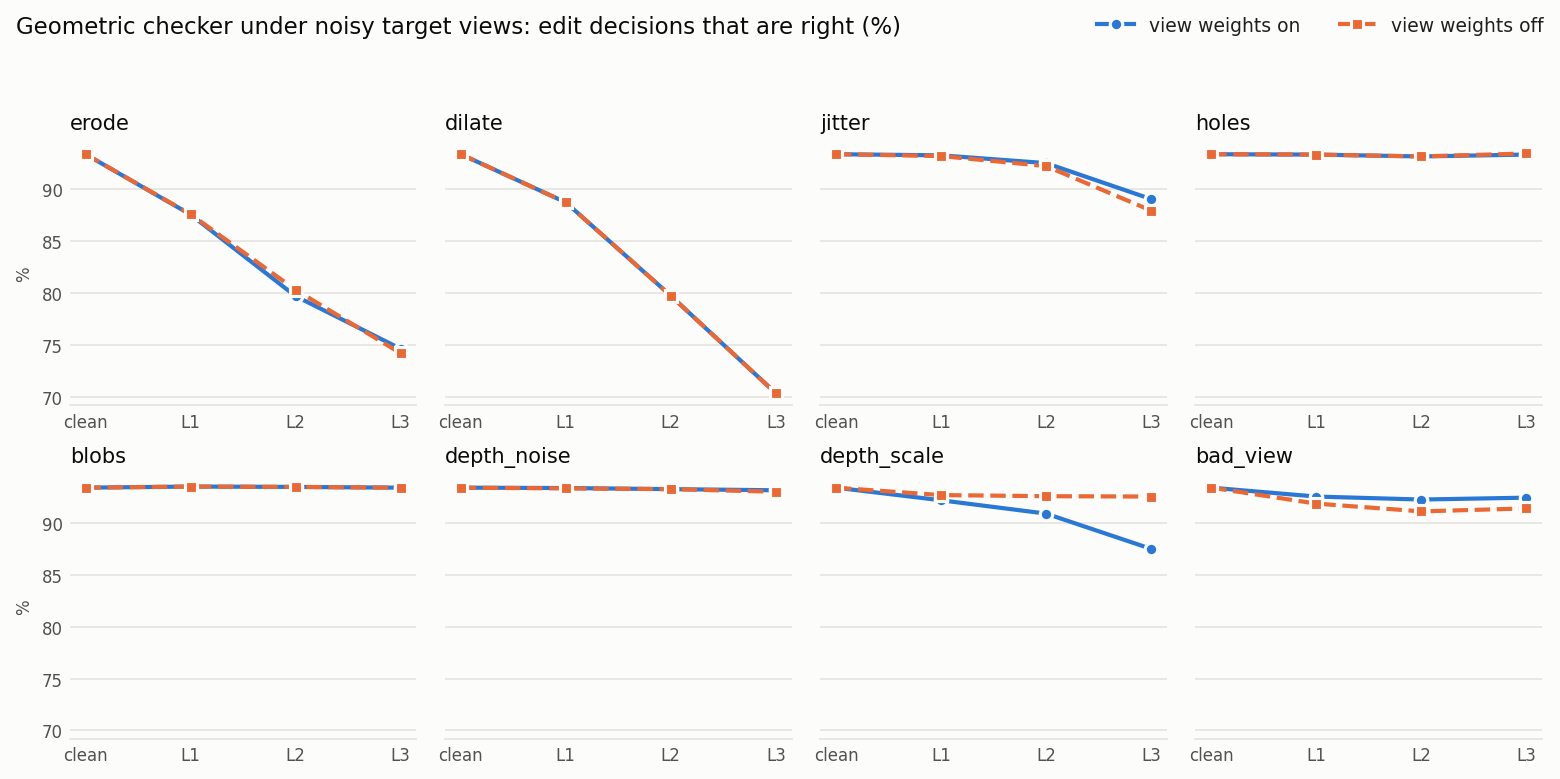
\includegraphics[width=\linewidth]{stage2_checker_accuracy.png}

  \small
  \begin{tabularx}{\linewidth}{@{}X r r@{}}
    \toprule
    \textbf{Condition (level 3)} & \textbf{Right} & \textbf{Harmful kept} \\
    \midrule
    clean views & 93\% & 4\% \\
    holes, blobs, depth noise & 93\% & 4\% \\
    one view shifted 32 px & 92\% & 4\% \\
    jitter 8 px & 89\% & 7\% \\
    depth scale $\pm$2\% (weights off: 93\%) & 87\% & 9\% \\
    erode 6 px & 75\% & 20\% \\
    dilate 6 px & \textbf{70\%} & \textbf{23\%} \\
    \bottomrule
  \end{tabularx}
  \normalsize

  \vspace{6pt}
  \noindent\colorbox{colorThree!12}{\parbox{\dimexpr\linewidth-2\fboxsep}{\small
    \textbf{Why dilation hurts most.} A mask 6 px too fat everywhere looks exactly like a
    slightly fatter object seen from every camera. The views still agree, so the weights
    stay at 1.00 and the bias goes straight into the score.}}

  \vspace{8pt}
  \placeholder{6cm}{Noise-tolerant rule}{Same chart with a rule that ignores a few pixels
    at the mask boundary and weighs silhouettes and depth separately. Source: W3.}
}

\block{Takeaways (draft)}{
  \begin{enumerate}
    \item On clean views the geometric gate is a strong judge: 93\% right decisions, rank
          correlation 0.89 with hidden 3D IoU.
    \item Random damage to the measurements cancels in the score difference; a systematic
          boundary bias does not.
    \item View weights catch inconsistent views, not consistent bias.
    \item \pending{Stage 1 headline from W1}
  \end{enumerate}

  {\scriptsize
  \begin{thebibliography}{9}\setlength{\itemsep}{0pt}
    \bibitem{gator} Q.~Wu et al., GATOR, arXiv:2610.11215, 2026.
    \bibitem{cadcodeverify} K.~Alrashedy et al., Generating CAD Code with
      Vision-Language Models for 3D Designs, ICLR 2025.
    \bibitem{cadrille} M.~Kolodiazhnyi et al., cadrille, ICLR 2026.
    \bibitem{sam3} N.~Carion et al., SAM 3, ICLR 2026.
    \bibitem{vggt} J.~Wang et al., VGGT, CVPR 2025.
  \end{thebibliography}}
}

\end{columns}
\end{document}
